\documentclass{article}\usepackage[]{graphicx}\usepackage[]{xcolor}
% maxwidth is the original width if it is less than linewidth
% otherwise use linewidth (to make sure the graphics do not exceed the margin)
\makeatletter
\def\maxwidth{ %
  \ifdim\Gin@nat@width>\linewidth
    \linewidth
  \else
    \Gin@nat@width
  \fi
}
\makeatother

\definecolor{fgcolor}{rgb}{0.345, 0.345, 0.345}
\newcommand{\hlnum}[1]{\textcolor[rgb]{0.686,0.059,0.569}{#1}}%
\newcommand{\hlsng}[1]{\textcolor[rgb]{0.192,0.494,0.8}{#1}}%
\newcommand{\hlcom}[1]{\textcolor[rgb]{0.678,0.584,0.686}{\textit{#1}}}%
\newcommand{\hlopt}[1]{\textcolor[rgb]{0,0,0}{#1}}%
\newcommand{\hldef}[1]{\textcolor[rgb]{0.345,0.345,0.345}{#1}}%
\newcommand{\hlkwa}[1]{\textcolor[rgb]{0.161,0.373,0.58}{\textbf{#1}}}%
\newcommand{\hlkwb}[1]{\textcolor[rgb]{0.69,0.353,0.396}{#1}}%
\newcommand{\hlkwc}[1]{\textcolor[rgb]{0.333,0.667,0.333}{#1}}%
\newcommand{\hlkwd}[1]{\textcolor[rgb]{0.737,0.353,0.396}{\textbf{#1}}}%
\let\hlipl\hlkwb

\usepackage{framed}
\makeatletter
\newenvironment{kframe}{%
 \def\at@end@of@kframe{}%
 \ifinner\ifhmode%
  \def\at@end@of@kframe{\end{minipage}}%
  \begin{minipage}{\columnwidth}%
 \fi\fi%
 \def\FrameCommand##1{\hskip\@totalleftmargin \hskip-\fboxsep
 \colorbox{shadecolor}{##1}\hskip-\fboxsep
     % There is no \\@totalrightmargin, so:
     \hskip-\linewidth \hskip-\@totalleftmargin \hskip\columnwidth}%
 \MakeFramed {\advance\hsize-\width
   \@totalleftmargin\z@ \linewidth\hsize
   \@setminipage}}%
 {\par\unskip\endMakeFramed%
 \at@end@of@kframe}
\makeatother

\definecolor{shadecolor}{rgb}{.97, .97, .97}
\definecolor{messagecolor}{rgb}{0, 0, 0}
\definecolor{warningcolor}{rgb}{1, 0, 1}
\definecolor{errorcolor}{rgb}{1, 0, 0}
\newenvironment{knitrout}{}{} % an empty environment to be redefined in TeX

\usepackage{alltt}
\usepackage{amsmath} %This allows me to use the align functionality.
                     %If you find yourself trying to replicate
                     %something you found online, ensure you're
                     %loading the necessary packages!
\usepackage{amsfonts}%Math font
\usepackage{graphicx}%For including graphics
\usepackage{hyperref}%For Hyperlinks
\usepackage[shortlabels]{enumitem}% For enumerated lists with labels specified
                                  % We had to run tlmgr_install("enumitem") in R
\hypersetup{colorlinks = true,citecolor=black} %set citations to have black (not green) color
\usepackage{natbib}        %For the bibliography
\setlength{\bibsep}{0pt plus 0.3ex}
\bibliographystyle{apalike}%For the bibliography
\usepackage[margin=0.50in]{geometry}
\usepackage{float}
\usepackage{multicol}

%fix for figures
\usepackage{caption}
\newenvironment{Figure}
  {\par\medskip\noindent\minipage{\linewidth}}
  {\endminipage\par\medskip}
\IfFileExists{upquote.sty}{\usepackage{upquote}}{}
\begin{document}

\vspace{-1in}
\title{Lab 5 -- MATH 240 -- Computational Statistics}

\author{
  Jake Schneider \\
  Colgate University  \\
  Department of Mathematics  \\
  {\tt jdschneider@colgate.edu}
}

\date{2/27/2025}

\maketitle

\begin{multicols}{2}
\begin{abstract}
This study seeks to determine which band among Manchester Orchestra, The Front Bottoms, or All Get Out had the greatest influence on their collaborative song ``Allentown". In an attempt to answer this question we gathered and analyzed musical metrics from 180 songs released prior to ``Allentown". With these metrics we constructed multiple box plots, which suggested that Manchester Orchestra had the most significant impact on this collaboration. 

\end{abstract}

\noindent \textbf{Keywords:} Data Summary; Collecting and Cleaning Data; Data Visualization

\section{Introduction}
In this lab we start attempting to analyze the contributing influences on the song ``Allentown" by The Front Bottoms, All Get Out and Manchester Orchestra. The 180 songs that we analyzed consisted of all releases before ``Allentown" except for joint albums, live albums, and single releases contained in a full album or an Extended Play. To aid our analysis, we used Essentia \citep{essentia}, Essentia Models \citep{essentiamodels} and The Lingusitic Inquiry and Word Count(LIWC) \citep{LIWC} to aid our analysis of each song. Essentia, an open source musical analysis tool, allowed us do a spectrogram analysis. Essentia Models provided insight into the sounds of the song in human terms(e.g., happy, sad, angry), and LIWC was used to analyze the lyrics. Using each analysis tool we were able to gather summary statistics on a variety of features for each band which we then compared to ``Allentown". This comparison allowed us to extract certain features which will help us to answer our question of which band had the most significant impact. 

\subsection{Musical Feature Definitions}
To quantify our question we examined several musical features. A key feature, spectral energy, was utilized in various forms throughout our study and focuses on the analyzing the frequency spectrum of audio signals and their various components. Along with spectral energy there are a few other relevant features that we need to define. 
\begin{itemize}\itemsep0em
\item Average Loudness: Average level of volume for a song.
\item Barkband Kurtosis: The distribution of spectral energy within certain frequency ranges that the human auditory system can perceive.
\item Chord Strength: Evaluation of the harmony and its role in the structure of the melody.
\item Dissonance: Measure the clash or tension between certain notes.
\item Dynamic Complexity: The variation in the rhythm and loudness.
\item Positive Words: The number of positive words in the lyrics. 
\item Perception: The frequency of spatial and directional words in the lyrics(e.g., in, out, up).
\item Spectral Centroid: Measures the brightness in the music which helps with genre classification.
\item Spectral Kurtosis: The shape of the spectral energy distribution which helps with genre classification.
\item Spectral Rolloff: Distinguishes between music and speech.
\item Spectral Skewness: The skewness of the spectral energy distribution.
\item Arousal: A songs ability to stimulate dopamine release for the listener. 
\end{itemize}

\section{Methods}
Our data set contained both numerical and categorical variables. 
The Essentia data that we extracted from the songs was contained in \texttt{.JSON} files, while the other two data sets were \texttt{CSV} files. In order to extract the Essentia \citep{essentia} data from the \texttt{.JSON} files we utilized the \texttt{stringr} package \citep{stringr} and the \texttt{jsonlite} package \citep{jsonlite}. The {\tt{fromJSON()}} function gave us a large list, which we converted to a data frame using \verb|for()| loops. The extracted variables included overall loudness, spectral energy, dissonance, pitch salience, tempo in beats per minute (bpm), beat loudness, danceability, and tuning frequency. Once we loaded both \texttt{EssentiaModelOutput.csv} and \texttt{LIWCOutput.csv} we had three data frames of raw information. 
 
\subsection{Cleaning and Merging \texttt{CSV} File Data}
To clean the \texttt{EssentiaModelOutput.csv} data we computed the averages for valence, arousal, happy mood, party mood, relaxed mood, sad mood, acoustic, electric, and instrumental. We removed all other columns keeping only these averages along with artist, album and song. The LIWC \texttt{CSV} was left unchanged. The simplest way to analyze our data was by merging the three data sets. 

Using the \verb|merge()| function we were able to merge our original data frame and the two {\texttt{CSV}} files that we downloaded. To prevent any duplicate rows, we matched the artist, album and track columns, ensuring the new data frame still had 181 rows. To analyze ``Allentown" separately from all other tracks we created two new \texttt{CSV} files, one with only ``Allentown" and another for all other songs, which allowed us to now create our summary statistics to start our analysis. 

\subsection{Creating Summary Stats}
To determine if ``Allentown" showcased unusual characteristics, we created a five number summary for each band to, comparing each of their feature ranges to ``Allentown". Before creating the five number summary we made sure to filter out any column that did not contain a numerical value. With all of our numerical values summarized we used the \verb|mutate()| function to create a new column to indicate the that the band was either out of range, unusual or within range for a given feature.
\begin{itemize}\itemsep0em
\item Out of Range: If ``Allentown" was below the minimum or above the maximum values of the band.
\item Unusual: If ``Allentown" was between the minimum and 25th percentile or between the maximum and 75th percentile
\item Within Range: If ``Allentown was between the 25th and 75th percentile. 
\end{itemize}

\subsection{Selecting Features and Plotting Data}
We filtered features to identify cases where only one band remained within range while the other two were either unusual or out of range. We took this approach because if all three bands fell within range on a feature, we would not be able to easily identify if one band had a stronger influence. Furthermore, if all three were out of range this also would not provide any meaningful insight. Focusing on features where only one band is in range helps us to determine which band could have had the most influence on that feature. This filtering process left us with 21 potential features, from which we randomly selected 12 for plotting and analysis. The 12 are as follows: arousal, average loudness, barkband kurtosis, chord strength, dissonance, dynamic complexity, perception, positive words, spectral centroid, spectral kurtosis, spectral rolloff and spectral skewness. We then used a box plot for each feature and plotted the ``Allentown" values against each of the box plots to help visually compare the values. 

\section{Results}
To answer our question of which band had the biggest impact on the song ``Allentown", we analyzed our box plots (Figure \ref{plot1}) and our numerical comparisons (Table \ref{compared.features}). By examining which features aligned with each ``Allentown" value, we can start to identify a trend. For average loudness, barkband kurtosis, chord strength, dissonance, perception, spectral centroid, spectral kurtosis, spectral rolloff and spectral skewness, Manchester Orchestra feature values are within range while All Get Out and The Front Bottoms feature values are out of range. This suggest that Manchester Orchestra had a more substantial impact on these features of the song, as these values would be considered outliers for the other two bands. When analyzing arousal we can see that the value for ``Allentown" falls within range for all 3 bands. However, this value falls within Manchester Orchestra first quartile and third quartile indicating that it most closely aligns with their typical song characteristics. A similar pattern is seen with dynamic complexity, where ``Allentown" falls within range for both All Get Out and Manchester Orchestra, but with ``Allentown" being in between the first and third quartile this could suggest a stronger influence. For the last feature, positive words, we see that The Front Bottoms are in range while the other two bands are out of range indicating that The Front Bottoms had a more substantial impact on this lyrical feature of the song. When analyze all 12 graphs, shown in we can see that Manchester Orchestra is in range 9 out of 12 times(Figure \ref{plot1}) indicating that overall they had the greatest impact to the song ``Allentown".

\section{Discussion}
Our analysis suggest that Manchester Orchestra had the most significant influence on ``Allentown", as 9 of the 12 features that we analyzed aligned with Manchester Orchestra. However, there are several limitations to our analysis that we need to consider. Our analysis ended up focusing mostly on the musical characteristics of ``Allentown", meaning that we fail to acknowledge that one band could have played a bigger role in the composition of the song. This is important to consider as some may argue that the composition of the song is a stronger measure of influence compared to the sonic resemblance.

Furthermore, we combined all of the data without accounting for the differences in how the music extractors may analyze the songs. Separating our analysis may have provided a deeper insight to who contributed more but also might have left us with a data set of insufficient size. Ultimately, while trying to determine who had the greatest impact on ``Allentown" is inherently subjective, our results indicate that its sonic profile most closely aligns with Manchester Orchestra.  


%%%%%%%%%%%%%%%%%%%%%%%%%%%%%%%%%%%%%%%%%%%%%%%%%%%%%%%%%%%%%%%%%%%%%%%%%%%%%%%%
% Bibliography
%%%%%%%%%%%%%%%%%%%%%%%%%%%%%%%%%%%%%%%%%%%%%%%%%%%%%%%%%%%%%%%%%%%%%%%%%%%%%%%%
\vspace{1em}


\begin{tiny}
\bibliography{bib}
\end{tiny}

\end{multicols}

%%%%%%%%%%%%%%%%%%%%%%%%%%%%%%%%%%%%%%%%%%%%%%%%%%%%%%%%%%%%%%%%%%%%%%%%%%%%%%%%
% Appendix
%%%%%%%%%%%%%%%%%%%%%%%%%%%%%%%%%%%%%%%%%%%%%%%%%%%%%%%%%%%%%%%%%%%%%%%%%%%%%%%%
\section{Appendix}

\begin{figure}[H]
  \begin{center}
  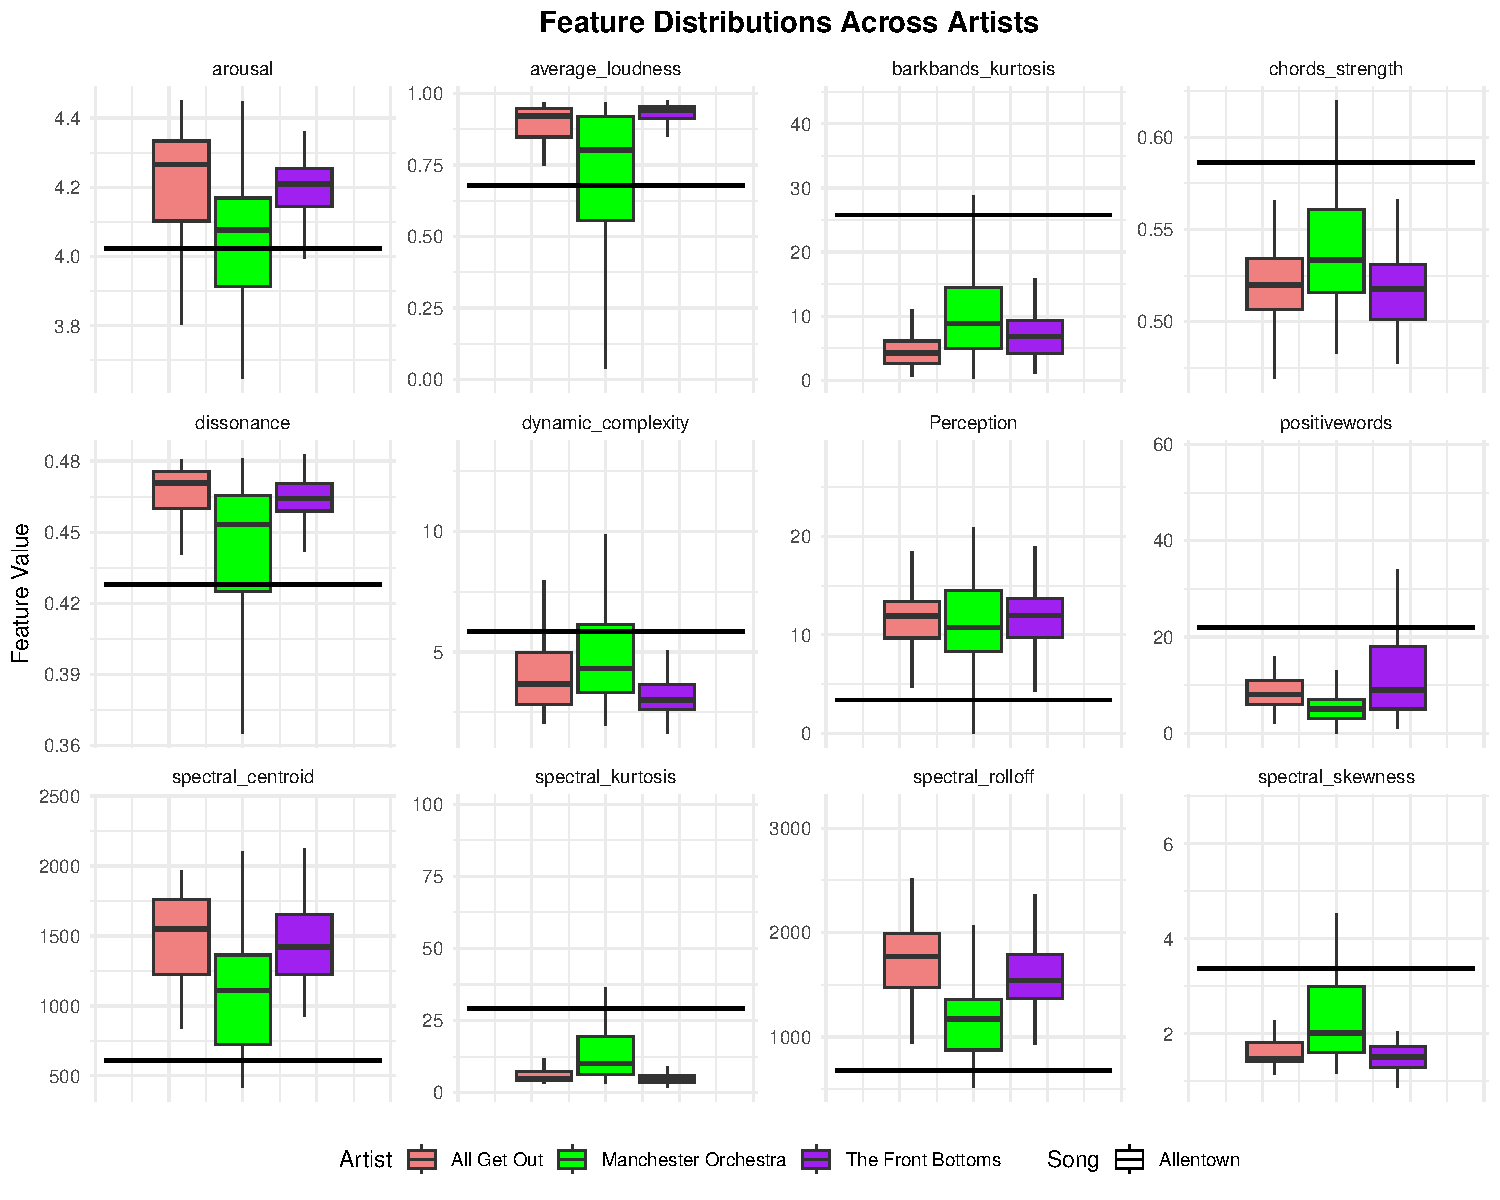
\includegraphics[width=\textwidth]{feature.plot.pdf}
  \caption{Features Box Plot}
  \label{plot1}
  \end{center}
\end{figure}


\begin{table}[ht]
\centering
\begin{tabular}{rlrrrrll}
  \hline
 & artist & min & LF & UF & max & description & feature \\ 
  \hline
1 & All Get Out & 1.14 & 0.81 & 2.42 & 4.12 & Outlying & spectral\_skewness \\ 
  2 & Manchester Orchestra & 1.16 & -0.49 & 5.09 & 6.75 & Within Range & spectral\_skewness \\ 
  3 & The Front Bottoms & 0.87 & 0.63 & 2.40 & 2.04 & Out Of Range & spectral\_skewness \\ 
  4 & All Get Out & 935.91 & 701.91 & 2767.30 & 2520.04 & Out Of Range & spectral\_rolloff \\ 
  5 & Manchester Orchestra & 518.87 & 151.27 & 2083.17 & 2566.67 & Within Range & spectral\_rolloff \\ 
  6 & The Front Bottoms & 927.04 & 740.58 & 2421.46 & 3190.29 & Out Of Range & spectral\_rolloff \\ 
  7 & All Get Out & 3.03 & -0.36 & 11.90 & 40.10 & Outlying & spectral\_kurtosis \\ 
  8 & Manchester Orchestra & 3.36 & -13.58 & 39.36 & 98.58 & Within Range & spectral\_kurtosis \\ 
  9 & The Front Bottoms & 1.89 & 0.00 & 9.55 & 10.47 & Out Of Range & spectral\_kurtosis \\ 
  10 & All Get Out & 836.21 & 419.54 & 2569.37 & 1967.62 & Out Of Range & spectral\_centroid \\ 
  11 & Manchester Orchestra & 418.64 & -231.76 & 2322.30 & 2106.83 & Within Range & spectral\_centroid \\ 
  12 & The Front Bottoms & 924.40 & 584.67 & 2298.03 & 2412.48 & Out Of Range & spectral\_centroid \\ 
  13 & All Get Out & 2.02 & -0.40 & 8.19 & 7.96 & Within Range & dynamic\_complexity \\ 
  14 & Manchester Orchestra & 1.96 & -0.90 & 10.34 & 13.21 & Within Range & dynamic\_complexity \\ 
  15 & The Front Bottoms & 1.63 & 1.00 & 5.26 & 6.50 & Outlying & dynamic\_complexity \\ 
  16 & All Get Out & 0.40 & 0.44 & 0.50 & 0.48 & Outlying & dissonance \\ 
  17 & Manchester Orchestra & 0.37 & 0.36 & 0.53 & 0.48 & Within Range & dissonance \\ 
  18 & The Front Bottoms & 0.43 & 0.44 & 0.49 & 0.48 & Out Of Range & dissonance \\ 
  19 & All Get Out & 0.62 & -2.65 & 11.38 & 17.68 & Out Of Range & barkbands\_kurtosis \\ 
  20 & Manchester Orchestra & 0.22 & -9.46 & 28.87 & 43.71 & Within Range & barkbands\_kurtosis \\ 
  21 & The Front Bottoms & 1.14 & -3.58 & 17.15 & 23.90 & Out Of Range & barkbands\_kurtosis \\ 
  22 & All Get Out & 0.16 & 0.70 & 1.10 & 0.97 & Outlying & average\_loudness \\ 
  23 & Manchester Orchestra & 0.00 & 0.01 & 1.46 & 0.97 & Within Range & average\_loudness \\ 
  24 & The Front Bottoms & 0.55 & 0.85 & 1.02 & 0.98 & Outlying & average\_loudness \\ 
  25 & All Get Out & 0.47 & 0.47 & 0.58 & 0.59 & Outlying & chords\_strength \\ 
  26 & Manchester Orchestra & 0.48 & 0.45 & 0.63 & 0.62 & Within Range & chords\_strength \\ 
  27 & The Front Bottoms & 0.48 & 0.46 & 0.58 & 0.57 & Out Of Range & chords\_strength \\ 
  28 & All Get Out & 3.80 & 3.76 & 4.68 & 4.45 & Within Range & arousal \\ 
  29 & Manchester Orchestra & 3.65 & 3.53 & 4.55 & 4.45 & Within Range & arousal \\ 
  30 & The Front Bottoms & 3.88 & 3.98 & 4.42 & 4.44 & Within Range & arousal \\ 
  31 & All Get Out & 4.67 & 4.14 & 18.91 & 20.89 & Out Of Range & Perception \\ 
  32 & Manchester Orchestra & 0.00 & -1.06 & 23.87 & 28.37 & Within Range & Perception \\ 
  33 & The Front Bottoms & 4.27 & 3.74 & 19.66 & 22.56 & Out Of Range & Perception \\ 
  34 & All Get Out & 2.00 & -1.50 & 18.50 & 58.00 & Outlying & positivewords \\ 
  35 & Manchester Orchestra & 0.00 & -3.00 & 13.00 & 27.00 & Outlying & positivewords \\ 
  36 & The Front Bottoms & 1.00 & -14.50 & 37.50 & 34.00 & Within Range & positivewords \\ 
   \hline
\end{tabular}
\caption{Artist Features Being Compared to Allentown} 
\label{compared.features}
\end{table}



\onecolumn






\end{document}
